\documentclass[10pt]{article}
\usepackage{geometry}                % See geometry.pdf to learn the layout options. There are lots.
\geometry{letterpaper}                   % ... or a4paper or a5paper or ... 
%\geometry{landscape}                % Activate for for rotated page geometry
%\usepackage[parfill]{parskip}    % Activate to begin paragraphs with an empty line rather than an indent

%%%%%%%%%%%%%%%%%%%%
\usepackage{natbib}
\usepackage[spanish]{babel}
\usepackage{xcolor}
\usepackage{url}
\usepackage{hyperref}
\usepackage{mathtools}


\title {Role Interviews Documentation}
\author{Echo Octubre \\
}
\date{{\bf Project Mini Description}: Aqui va la descripcion del producto.}
%\date{}                                           % Activate to display a given date or no date

\begin{document}
\maketitle
Macias Gomez Jorge 

\section{Personality insights}
    \subsection{Modelos de personalidad}
        El servicio Personality Insights deduce características de personalidad basándose en tres modelos primarios:\\
        Las cinco grandes características de personalidad representan el modelo más utilizado para describir de forma general cómo interactúa una persona con el mundo. El modelo incluye cinco dimensiones primarias: \\
        Simpatía, Responsabilidad, Extraversión, Rango emocional, y Apertura.Cada dimensión tiene seis facetas que caracterizan más a un individuo según la dimensión.\\
    
        \subsubsection{Simpatía}
                Es la tendencia de una persona a ser compasiva y cooperadora con los demás.\\                \textbf{Facetas:} \\
                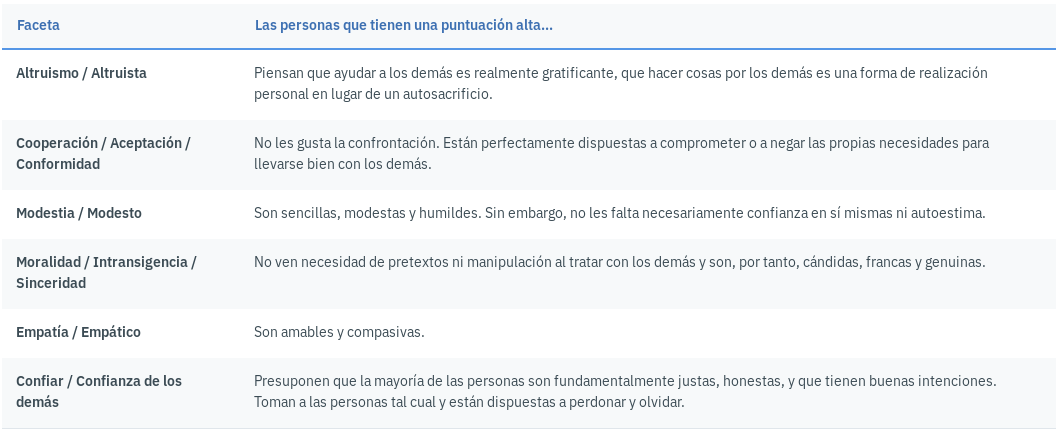
\includegraphics[scale=.37]{FacetasSimpatia.png}\\
               \textbf{ Que significan los valores}:\\ 
                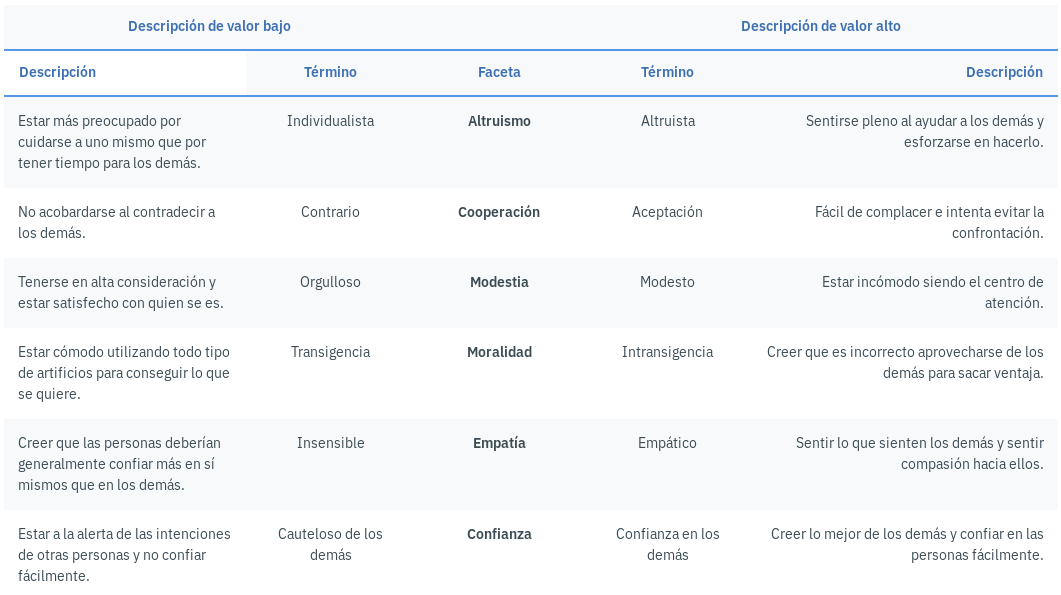
\includegraphics[scale=.37]{AltoBajoSimpatia.png}\\
                
        \subsubsection{Responsabilidad}
                Responsabilidad es la tendencia de una persona a actuar de forma organizada o meticulosa.\\                
                \textbf{Facetas:}\\
                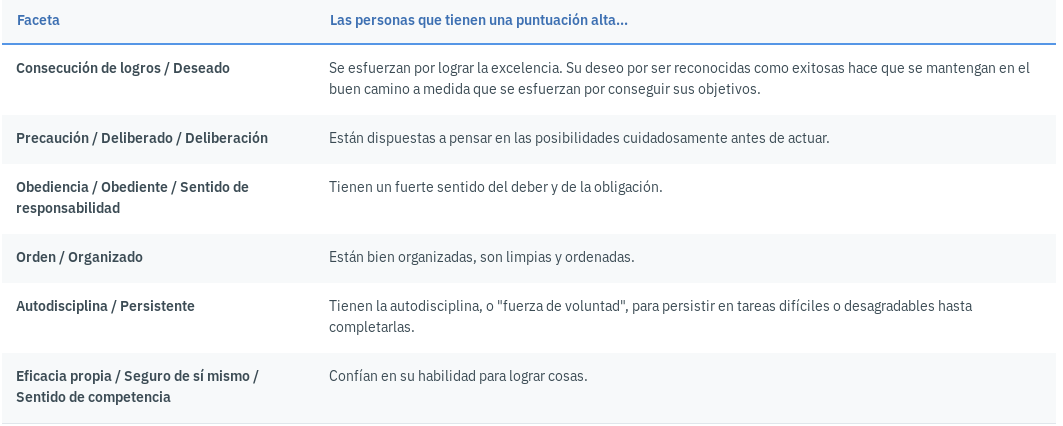
\includegraphics[scale=.37]{FacetasResponsabilidad.png}\\
                \textbf{Que significan los valores:}\\ 
                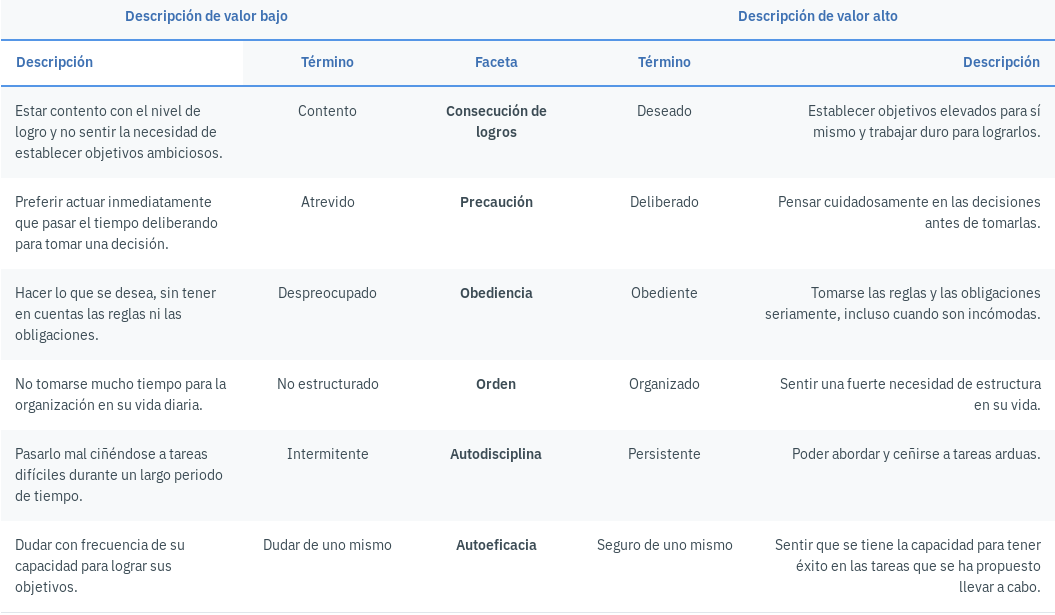
\includegraphics[scale=.37]{AltoBajoResponsabilidad.png}\\
                
        \subsubsection{Extraversión}
                Extraversión es la tendencia de una persona a buscar la estimulación en compañía de los demás.\\                
                \textbf{Facetas:}\\
                \includegraphics[scale=.37]{FacetasExtraversion.png}\\
                \textbf{Que significan los valores:}\\ 
                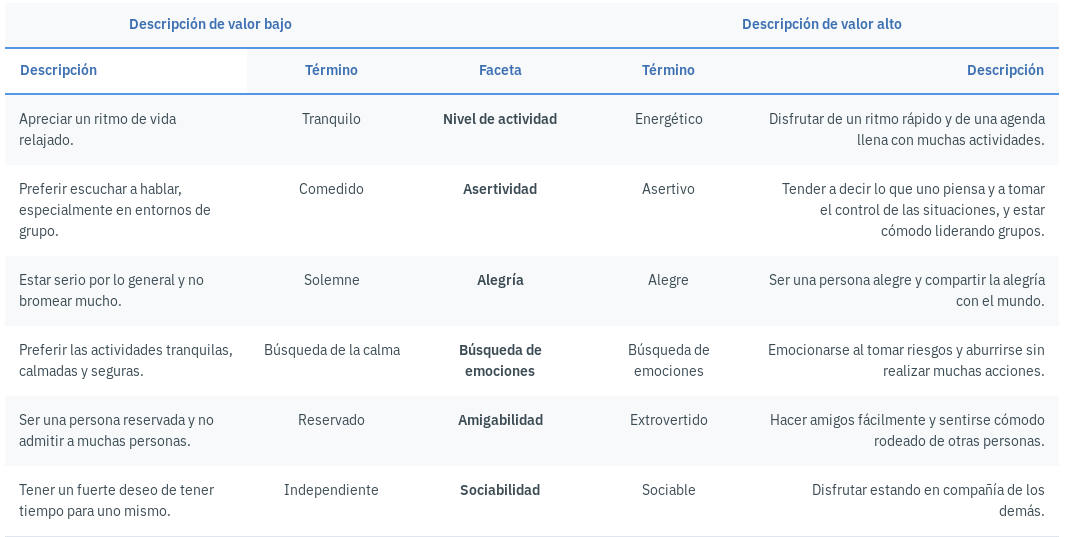
\includegraphics[scale=.37]{AltoBajoExtraversion.png}\\
        
        \subsubsection{Rango emocional}
                Rango emocional, también conocido como Neurosis o Reacciones naturales, es el punto hasta el que las emociones de una persona son sensibles al entorno del individuo.\\
                
                \textbf{Facetas:}\\
                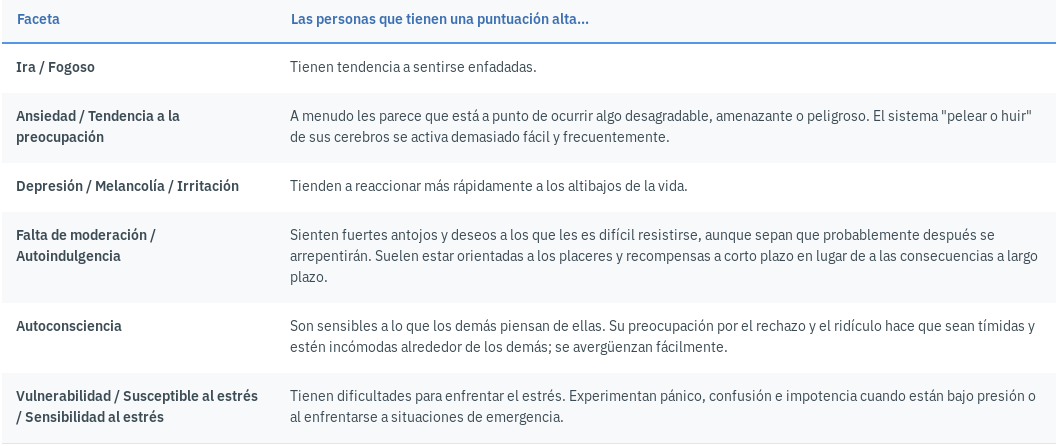
\includegraphics[scale=.37]{FacetasRangoEmocional.png}\\
                \textbf{Que significan los valores:}\\ 
                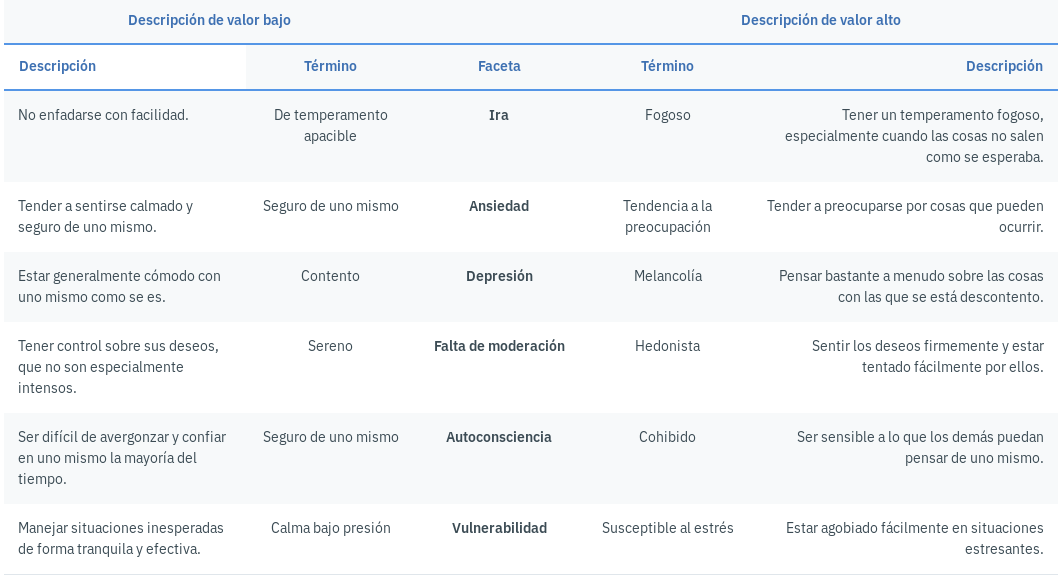
\includegraphics[scale=.37]{AltoBajoRangoEmocional.png}\\
                
        \subsubsection{Apertura}
                Apertura, o Abierto a la experiencia, es el punto hasta el que una persona está abierta a experimentar actividades diversas.\\
                
                \textbf{Facetas:}\\
                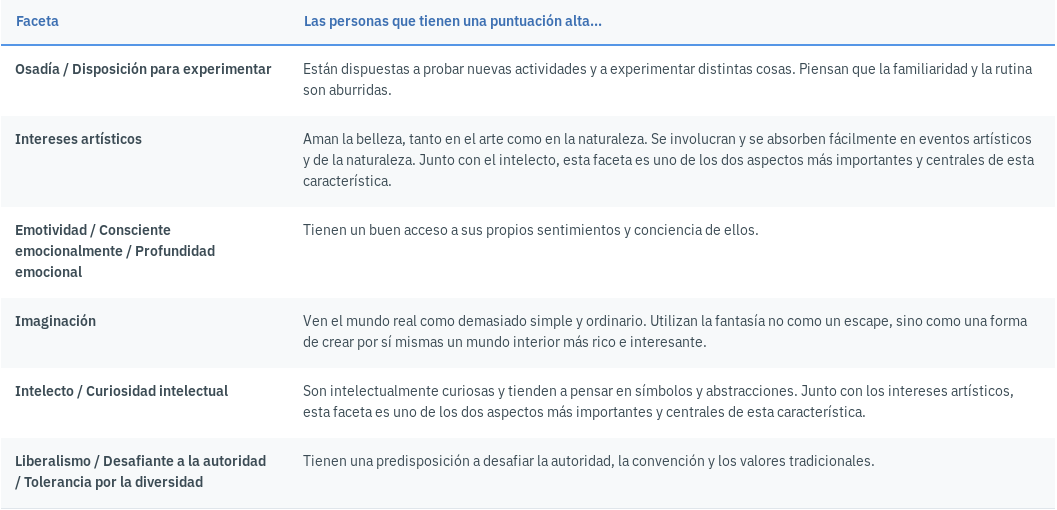
\includegraphics[scale=.37]{FacetasApertura.png}\\
                \textbf{Que significan los valores:}\\ 
                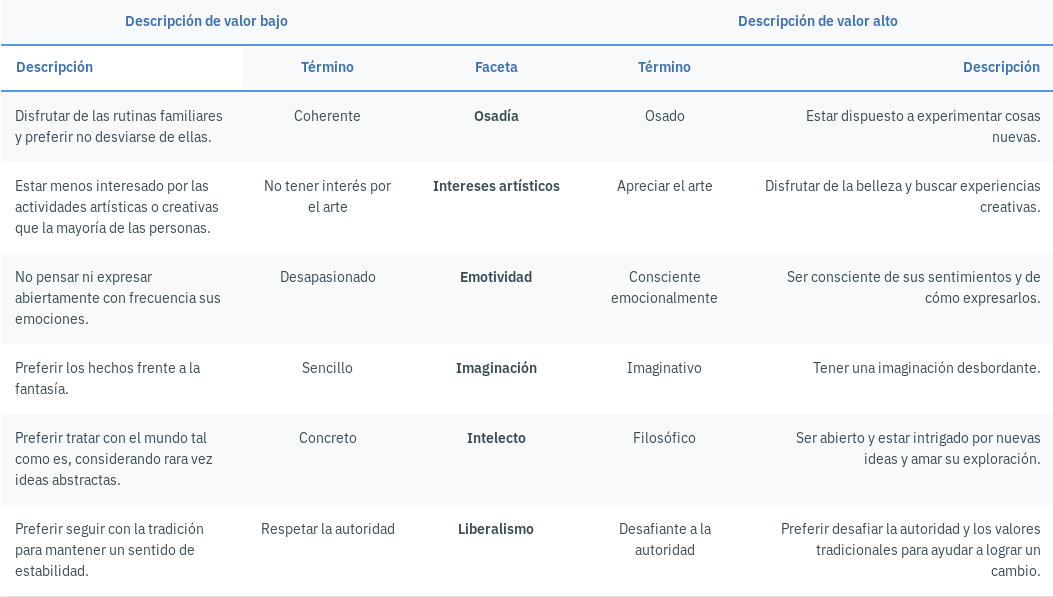
\includegraphics[scale=.37]{AltoBajoApertura.png}\\
                
                
                
                
                
    \subsection{Correlaciones entre los 5 grandes}
            \textbf{Simpatia vs All} \\
            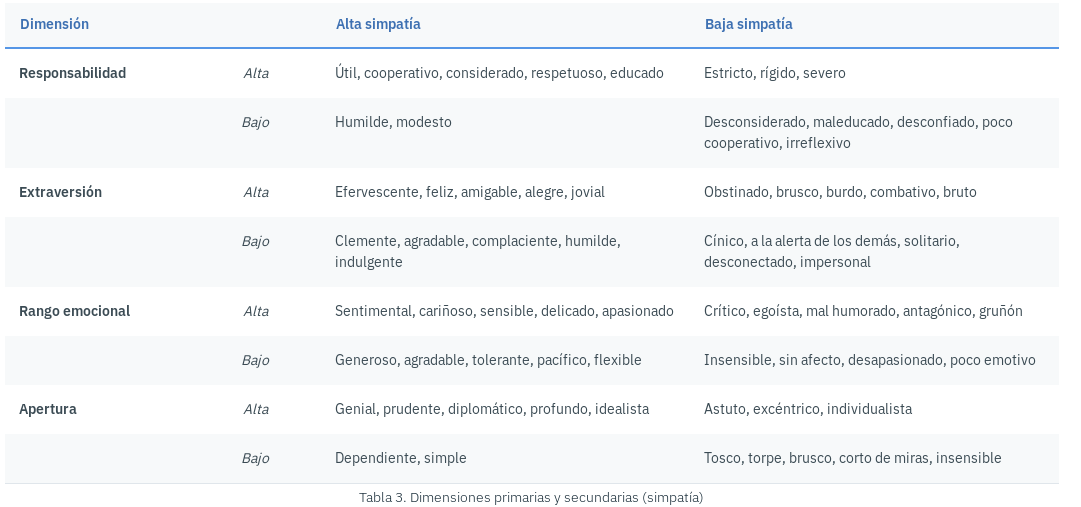
\includegraphics[scale=.37]{simpatiavsall.png}\\
            \textbf{Responsabilidad vs All} \\
            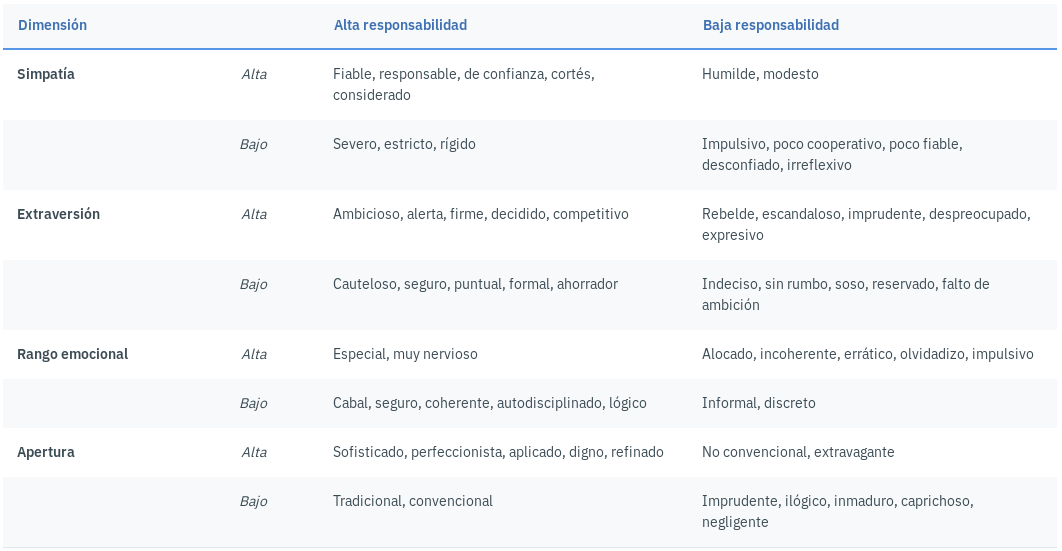
\includegraphics[scale=.37]{ResponsabilidadvsAll.png}\\
            \textbf{Extraversion vs All} \\
            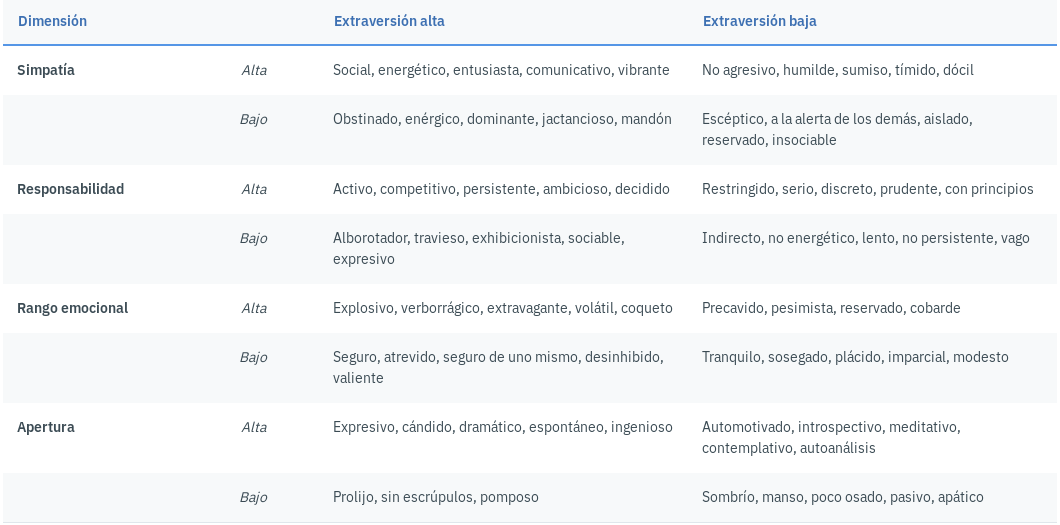
\includegraphics[scale=.37]{ExtraversionvsAll.png}\\
            \textbf{Rango Emocional vs All} \\
            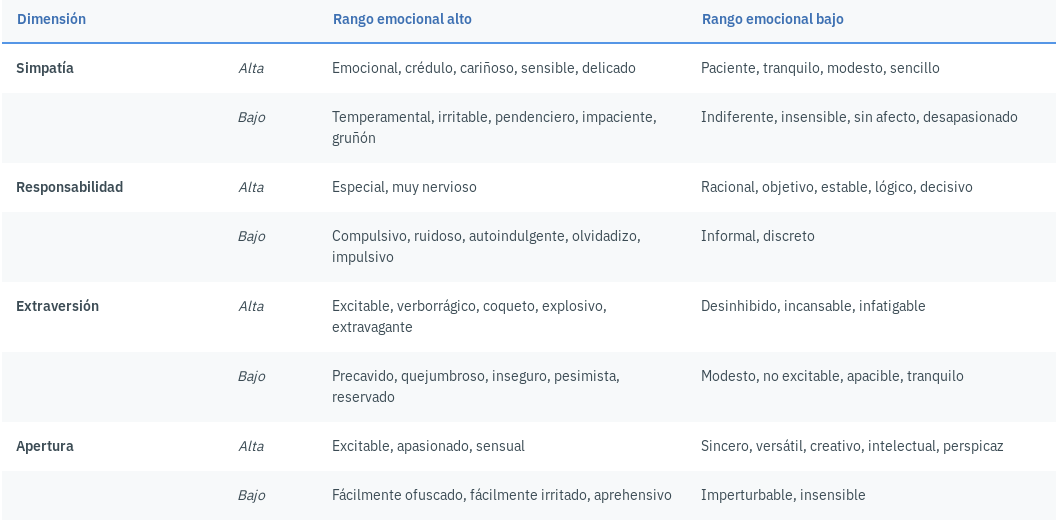
\includegraphics[scale=.37]{RangoEmocionalvsAll.png}\\
                        
                
                
                
                
                
                
        
        
    \subsection{Necesidades}
         Necesidades describe los aspectos de un producto con los que es probable que se identifique una persona. El modelo incluye doce necesidades características: \\
         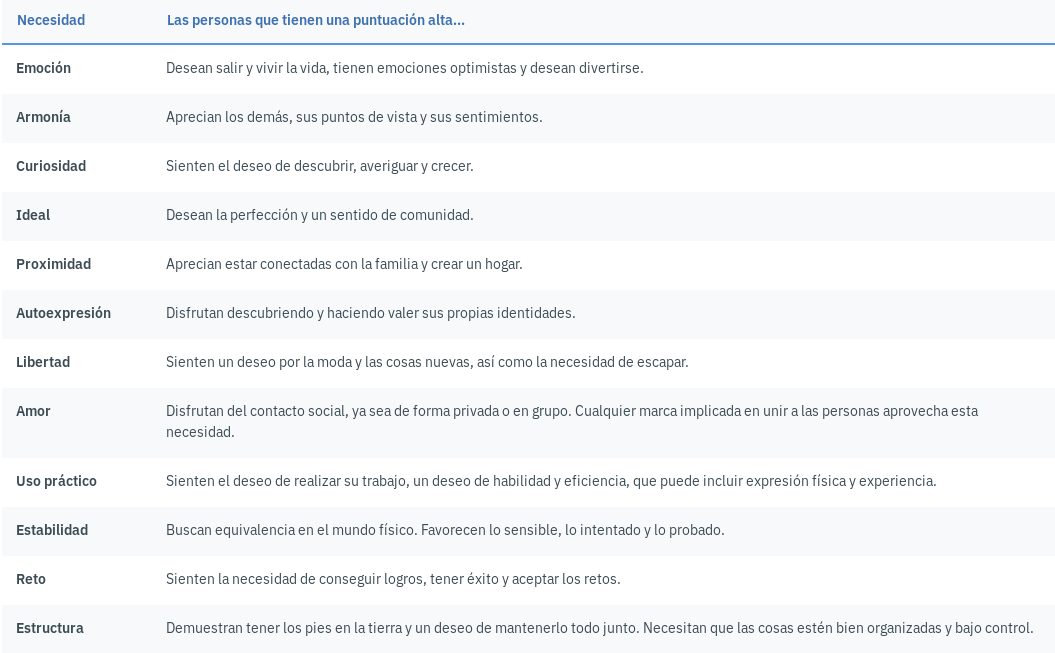
\includegraphics[scale=.37]{Necesidades.png}
         
         
    
    \subsection{Valores}
          Valores describe los factores de motivación que influyen en la toma de decisiones de una persona. El modelo incluye cinco valores: \\
          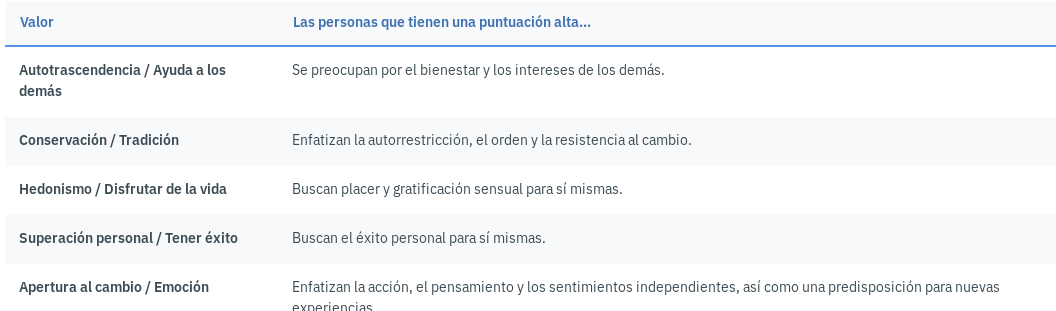
\includegraphics[scale=.37]{Valores.png}
          
          
          
          
          
          
        








\end{document}  
%%%%%%%%%%%%%%%%%%%%%%%%%%%%%%%%%%%%%%%%%%%%%%